\chapter{Framing and Switching}

\section{Framing}

\noindent
$\rightarrow$ Là quá trình đóng gói và mở gói dữ liệu ở hai đầu dây:

\begin{itemize}
    \item Receiver $\rightarrow$ cần phải tách dòng dữ liệu (bit stream) từ Physical Layer thành các khung (frame) để xử lý.
    \item Sender $\rightarrow$ đóng gói các tin từ Network Layer thành các khung trước khi đẩy xuống Physical Layer.
\end{itemize}
\medskip

\noindent
\underline{Self-note:} 
\medskip

\noindent
Tại sao cần phải framing?

\begin{itemize}
    \item[$\rightarrow$] Tầng vật lý chỉ biết truyền các tín hiệu điện/quang liên tục (bit 0 và 1) từ nơi gửi đến nơi nhận.
    \item[$\Rightarrow$] Không hề biết đâu là bắt đầu, đâu là kết thúc $\rightarrow$ chỉ là một dòng bit stream liên tục.
\end{itemize}
\medskip

\subsection{Frame Detection}

\noindent
Cách xác định ranh giới của frame $\rightarrow$ giúp máy thu nhận ra điểm bắt đầu và điểm kết thúc của một khung trong bit stream hỗn tạp ($\rightarrow$ the start of each frame needs to be marked).
\medskip

\noindent
\textbf{Các phương pháp để đánh dấu ranh giới các frame (frames' borders):}

\begin{itemize}
    \item Character count in the header (đếm ký tự trong phần header).
    \item Byte/Character stuffing (nhồi byte/ký tự).
    \item Bit stuffing (nhồi bit).
    \item Line code violation of Physical Layer with illegal signals (vi phạm mã đường truyền).
\end{itemize}

\subsubsection{Character Count in the Frame Header}

\noindent
\textbf{Nguyên lý hoạt động:}
\medskip

\noindent
Trong phần header của mỗi frame, bên gửi sẽ ghi rõ tổng số lượng bytes có trong khung đó.

$\Rightarrow$ Receiver đọc con số này $\rightarrow$ đếm đủ số lượng bytes thì biết được điểm kết thúc của frame đó.
\medskip

\noindent
\textbf{Ví dụ:} giao thức DDCMP (Digital Data Communications Message Protocol) của hãng DEC (Digital Equipment Corporation) ra đời năm 1974 sử dụng phương pháp này.
\medskip

\begin{figure}[h]
    \centering
    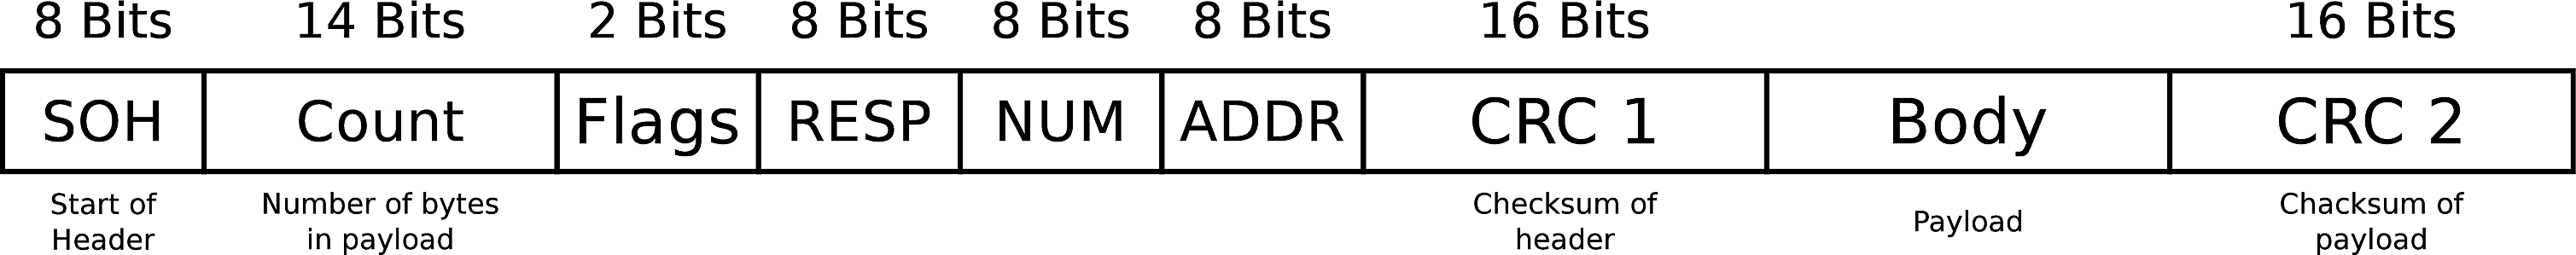
\includegraphics[width=1\textwidth]{assets/chap_3/char_count.png}
\end{figure}
\medskip

\noindent
Cấu trúc khung DDCMP:

\begin{itemize}
    \item Bắt đầu bằng \texttt{SOH} (Start of Header).
    \item Tiếp theo là field \texttt{Count} (14 bits) chứa số lượng byte trong khung.
    \item Sau đó là các field khác (như \texttt{Flags}, \texttt{Address}, ...) và cuối cùng là \texttt{Payload} (\texttt{Body}).
\end{itemize}
\medskip

\noindent
\textbf{Vấn đề (potential issue):}
\medskip

\noindent
Field \texttt{Count} bị nhiễu trên đường truyền.
\medskip

$\Rightarrow$ Receiver sẽ đếm sai điểm cuối của khung hiện tại (nó sẽ tưởng dài hơn hoặc ngắn hơn so với thực tế) $\rightarrow$ mất luôn cả phần đầu của khung kế tiếp do nhầm lẫn với phần cuối khung hiện tại.

$\Rightarrow$ Mất đồng bộ dây chuyền (desynchronization) $\rightarrow$ receiver không thể xác định đâu là điểm bắt đầu hay kết thúc của những khung sau đó nữa $\rightarrow$ error recovery sẽ rất phức tạp.
\medskip

\noindent
\underline{Self-note:}
\medskip

\noindent
Cứ tưởng tượng như mình là chủ kho và có ông giao hàng đến đưa mình tờ giấy ghi số lượng thùng hàng được lấy $\rightarrow$ nếu tờ giấy bị nhiễu thì mình sẽ không xác định rõ số lượng thùng hàng được lấy.
\medskip

\subsubsection{Control Sequences}

\noindent
\textbf{Chuỗi điều khiển (control sequences)} $\rightarrow$ là việc sử dụng các kí tự đặc biệt (gọi là sentinel characters - kí tự canh gác) để đánh dấu ranh giới của frame.

$\Rightarrow$ Thay vì điểm số lượng (như character count) $\rightarrow$ receiver sẽ truy các dòng bit liên tục cho đến khi gặp đúng kí tự đặc biệt này thì nó mới bắt đầu nhận hay kết thúc frame.
\medskip

\textbf{$\rightarrow$ Rủi ro:} nếu trong phần dữ liệu (data field) có xuất hiện các kí tự đặc biệt đó $\rightarrow$ receiver sẽ bị nhầm lẫn và tưởng đó là điểm kết thúc/bắt đầu của frame.

$\Rightarrow$ Giải pháp là sử dụng kĩ thuật nhồi byte/kí tự để phân biệt được.
\medskip

\subsubsection{Byte/Character stuffing}

\noindent
\textbf{Nguyên lý hoạt động:}

\begin{itemize}
    \item Sender $\rightarrow$ chèn (stuff) thêm kí tự vào dữ liệu để đánh dấu.
    \item Receiver $\rightarrow$ gỡ bỏ (destuff) các kí tự thừa đó để lấy lại dữ liệu gốc.
\end{itemize}
\medskip

\noindent
\textbf{Nhược điểm:}
\medskip

\noindent
$\rightarrow$ Phụ thuộc chặt chẽ vào bảng mã (strongly relationship with the character encoding):

\begin{itemize}
    \item \textbf{Yêu cầu:} phương pháp này bắt buộc hệ thống phải dùng một bảng mã cụ thể (chẳng hạn như ASCII) để định nghĩa.
    \item \textbf{Hạn chế:} nếu mình muốn truyền dữ liệu dùng bảng mã khác (ví dụ như Unicode 16-bit) hoặc dữ liệu nhị phân thuần túy (binary data) không theo chuẩn kí tự nào $\rightarrow$ phương pháp này sẽ gặp rắc rối.
\end{itemize}
\medskip

\noindent
$\rightarrow$ Các giao thức mới hơn của lớp này không còn hoạt động theo dạng byte (byte-oriented), mà chuyển sang dạng bit (bit-oriented).

$\Rightarrow$ Cách này cho phép sử dụng mọi kiểu mã hóa ký tự (allows using any character encoding) $\rightarrow$ không cần quan tâm kí tự điều khiển là gì.
\medskip

\subsubsection{Example: Byte/Character stuffing (BISYNC)}

\begin{figure}[h]
    \centering
    
\includegraphics[width=1\textwidth]{assets/chap_3/bisync.png}
\end{figure}
\medskip

\noindent
\textbf{Tổng quan:}

\begin{itemize}
    \item Tên đầy đủ $\rightarrow$ Binary Synchronous Communication (BISYNC - truyền thông đồng bộ nhị phân).
    \item Do IBM phát triển vào những năm 1960s.
    \item[$\rightarrow$] Là giao thức byte (character) oriented.
\end{itemize}
\medskip

\pagebreak

\noindent
\textbf{Các kí tự đặt biệt (special characters) cần nhớ:}

\begin{itemize}
    \item \texttt{SYN} (Synchronous Idle) $\rightarrow$ đánh dấu bắt đầu của một frame.
    \item \texttt{SOH} (Start of Header) $\rightarrow$ đánh dấu bắt đầu phần header.
    \item \texttt{STX} (Start of Text) $\rightarrow$ đánh dấu bắt đầu phần payload (phần dữ liệu chính).
    \item \texttt{ETX} (End of Text) $\rightarrow$ đánh dấu kết thúc phần payload.
    \item \texttt{DLE} (Data Link Escape) $\rightarrow$ kí tự thoát $\Rightarrow$ dùng để xử lý những trường hợp khác biệt (stuffing).
\end{itemize}
\medskip

\noindent
\textbf{Cơ chế stuffing:}
\medskip

\noindent
$\rightarrow$ Khi dữ liệu người dùng (body/payload) vô tình chứa các kí tự đặc biệt $\Rightarrow$ dùng \texttt{DLE} để có thể preserve được chúng:

\begin{itemize}
    \item \textbf{Nếu dữ liệu có \texttt{ETX}} $\rightarrow$ receiver sẽ tưởng là hết frame $\Rightarrow$ sender sẽ chèn thêm \texttt{DLE} vào trước $\rightarrow$ gửi đi \texttt{DLE ETX} $\rightarrow$ receiver sẽ hiểu được \texttt{ETX} này là dữ liệu.
    \item \textbf{Nếu dữ liệu có \texttt{DLE}} $\rightarrow$ receiver sẽ tưởng là bắt đầu kí hiệu thoát $\Rightarrow$ chèn thêm \texttt{DLE} vào trước (nhân đôi) $\rightarrow$ gửi đi \texttt{DLE DLE} $\rightarrow$ receiver sẽ hiểu được \texttt{DLE} này là dữ liệu.
\end{itemize}
\medskip

\noindent
\underline{Self-note:}
\medskip

\noindent
$\rightarrow$ Cứ nghĩ như trong C++, muốn in \texttt{"Hello World"} thì mình phải viết \texttt{\textbackslash"Hello World\textbackslash"} để thoát kí tự ngoặc kép vậy.
\medskip
